\chapter[Resultados Obtidos]{Resultados Obtidos}
Neste capítulo são exibidos os resultados obtidos desta arquitetura de extração.

\section{Arquitetura de Extração}
Para documentar o funcionamento da arquitetura de extração foi criado um diagrama de fluxo de dados, este representado na Figura \ref{image:diagramFlux}.
\begin{figure} [H]
\centering
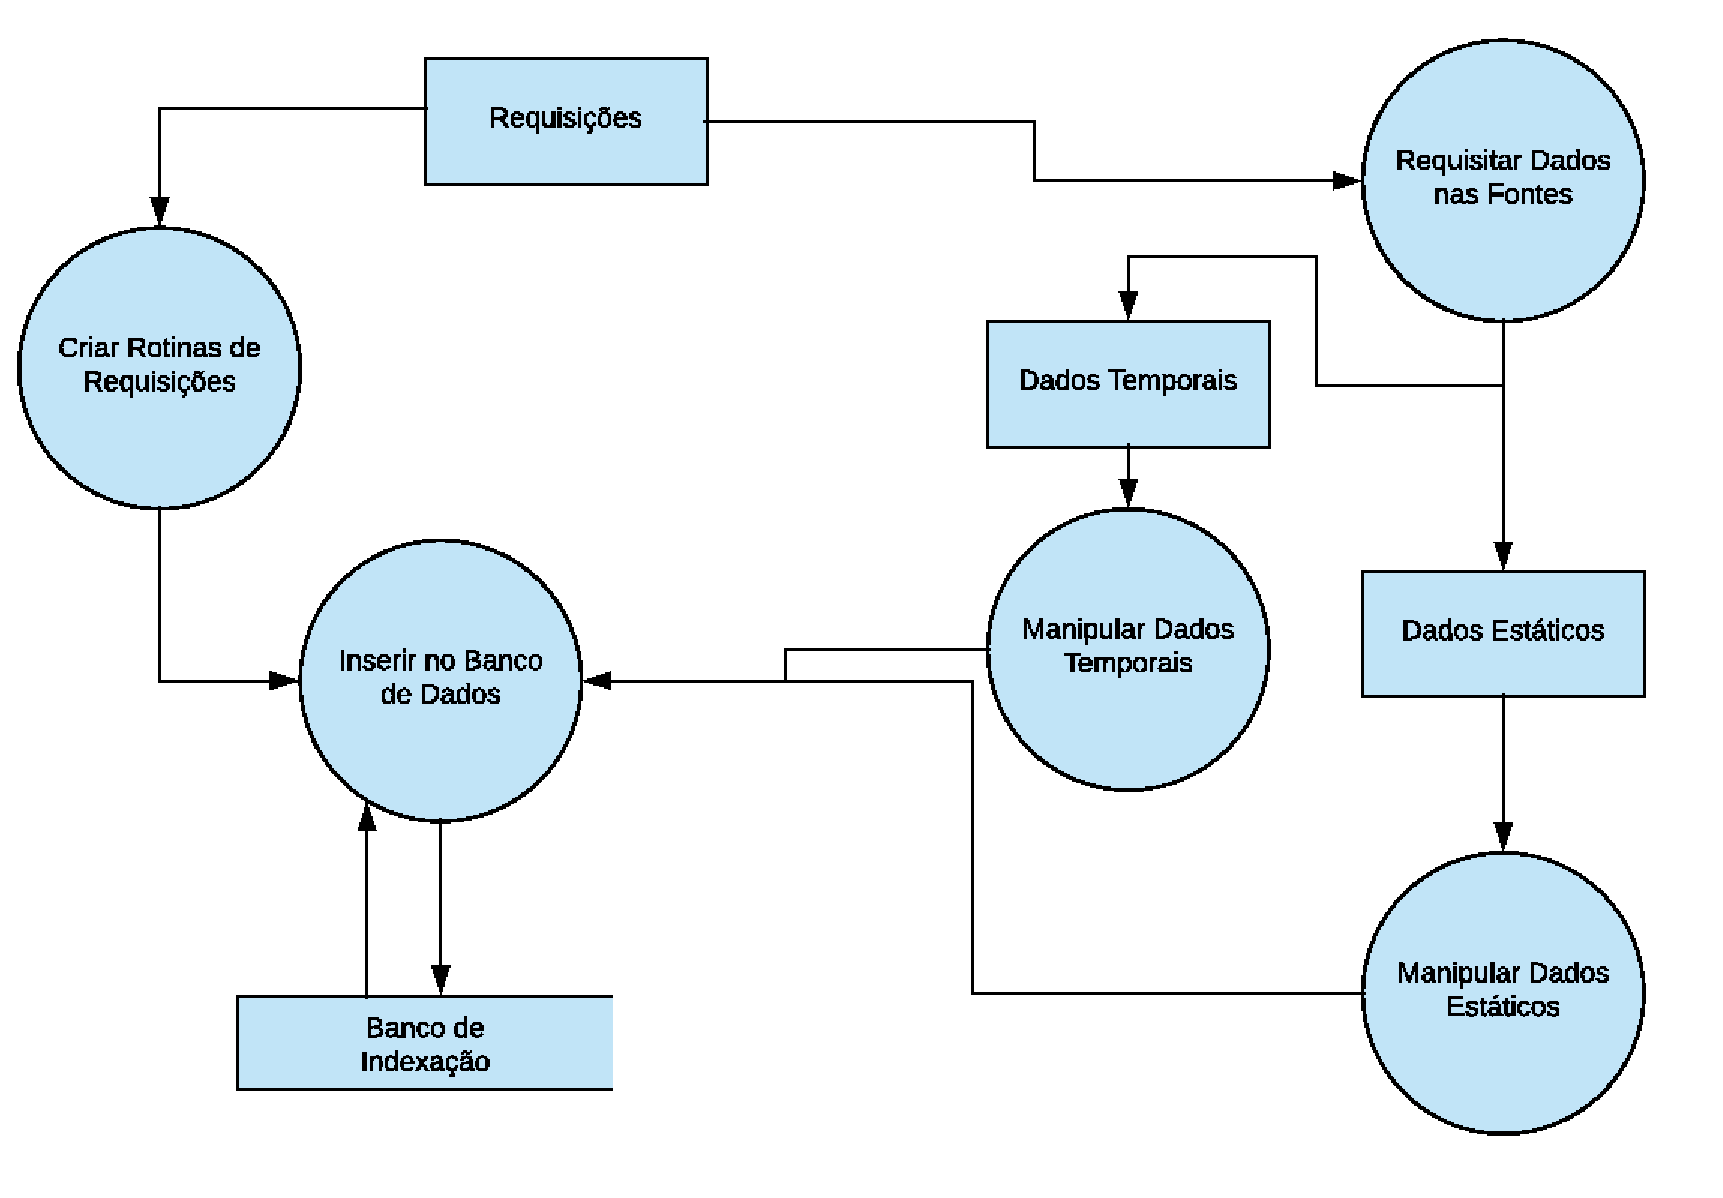
\includegraphics[scale=0.45]{figuras/diagramaFluxo.eps}
\caption{Diagrama de Fluxo de Dados}
\label{image:diagramFlux}
\end{figure}

Este diagrama possui três entidades, cinco processo e um armazenamento. As entidades representam as requisições que a arquitetura faz, os dados estáticos e temporais que serão manipulados. O armazenamento representa o banco de indexação onde estes dados serão inseridos.

O processo de \textbf{Requisitar Fontes de Dados} representa a funcionalidade da arquitetura de conseguir extrair dados de diversas fontes do mercado de jogos, para futuramente serem manipulados e inseridos no armazenamento.

O processo de \textbf{Criar Rotinas de Requisições} representa a funcionalidade da arquitetura de elaborar rotinas onde os dados temporais do armazenamento serão atualizados.

O processo de \textbf{Manipular Dados Estáticos} representa a funcionalidade da arquitetura de receber os dados da requisições, separar os que são estáticos, manipulá-los e prepará-los para a inserção no armazenamento.

O processo de \textbf{Manipular Dados Temporais} representa a funcionalidade da arquitetura de receber os dados da requisições, separar os que são temporais, manipulá-los e prepará-los para a inserção no armazenamento.

O processo de \textbf{Inserir no Banco de Dados} representa a funcionalidade da arquitetura de pegar os dados que foram manipulados e inseri-los no armazenamento.

\section{Software de Extração}
Seguindo a arquitetura proposta para a extração dos dados, foi verificado que a extração ocorria da maneira prevista, onde apenas nas primeiras 8 horas, foram recolhidos 8341 jogos. Porém, após as 8 horas passadas, foram identificados os gargalos da arquitetura. 

E não era de conhecimento, que a API do Youtube possuía limitações de requisições. Este foi o gargalo da arquitetura, pois passadas 8 horas, nenhum jogo mais era adicionado ao banco. Após isso foi feita uma mudança significativa no software de extração, há separação entre dois tipos, assim a primeira inserção, seria feita apenas com os dados estáticos, e as atualizações com os dados temporais.

Com o problema da primeira inserção resolvido, foi pensando em como seria contornado as limitações da API do Youtube, para isso foi pensado em duas soluções. Há primeira, a qual foi implementada, foi diminuir a frequência que estes dados era requisitados, e com isso tem-se mais tempo para o tratamento dos erros que ocorreram. 

A segunda seria a aquisição de diversas chaves da API, assim, seria feito uma alternância entre essas chaves para contornar as limitações da API, no momento da criação do projeto existiam 26.586 jogos no banco de dados da Steam, como cada chave insere aproximadamente 8 mil jogos, eram necessárias quatro chaves para fazer a inserção completa, porém, este tipo de abordagem possui seus problemas, pois para cada chave, era preciso ter um conta de desenvolvedor na Google Developers, por conseguinte quanto mais jogos houvesem, mais chaves seriam necessárias.

No tocante das limitações de requisições das outras APIs, como essas não atrapalhavam diretamente a inserção dos dados no Elasticsearch, a solução implementada é mais simples. Quando ocorre algum erro de alguma destas requisições, o id do jogo é guardado num arquivo, e futuramente, e realizada nova inserção dos jogos guardados no arquivo, caso ocorra erro novamente, o jogo é deletado.	

Após feita a divisão dos dados, foi possível notar que, para fazer a primeira inserção dos dados estáticos, foram inseridos 12.813 jogos, em 7 horas. Nota-se então que houve uma melhora na \textit{performace} do algoritmo implementado.

\section{Visualização dos Dados}
Nesta seção são mostrados alguns \textit{dashboards} criados com a ferramenta Kibana, possibilitando uma melhor visualização dos dados.

\subsection*{\textit{Dashboard} Total}
Neste \textit{dashboard} é mostrado as relações entre todos os jogos no banco de dados da Steam. Um exemplo deste \textit{dashboard} pode ser visto na Figura \ref{image:totalDash}.
\begin{figure} [H]
\centering
\includegraphics[scale=0.25]{figuras/totalDashboard.eps}
\caption{\textit{Dashboard} Total}
\label{image:totalDash}
\end{figure}

Neste \textit{dashboard} é possível notar que, há muito mais avaliações positivas que negativas, a partir do ano de 2013 a Steam, praticamente dobrou o número de jogos inseridos por ano, a cada ano. Também nota-se que a grande maioria dos jogos possuem suporte a língua inglesa e são feitos para plataforma Windows\footnote[1]{\url{https://www.microsoft.com/pt-br/windows}}. Outras métricas foram levantadas, como, gênero e categoria mais utilizado, desenvolvedora com mais jogos e meses com mais lançamentos.

\subsection*{\textit{Dashboard} de Gênero}
Neste \textit{dashboard} é mostrado as relações entre os jogos de um determinado gênero. Um exemplo deste \textit{dashboard} pode ser visto na Figura \ref{image:genreDash}.
\begin{figure} [H]
\centering
\includegraphics[scale=0.25]{figuras/genreDashboard.eps}
\caption{\textit{Dashboard} do Gênero Ação}
\label{image:genreDash}
\end{figure}

Neste \textit{dashboard} foi utilizado o gênero \textit{indie}, pois o mesmo e o mais utilizado na Steam, nele é possível notar que foram criados mais jogos \textit{indies} a partir do ano de 2013, coincidindo com o sucesso da Steam. Outras métricas foram levantadas, como, categorias, linguagens e plataformas mais utilizadas, desenvolvedora com mais jogos, meses com mais lançamentos e gêneros que mais foram utilizados em conjunto com o gênero \textit{indie}.

\subsection*{\textit{Dashboard} de Desenvolvedora}
Neste \textit{dashboard} é mostrado as informações de uma determinada desenvolvedora. Um exemplo deste \textit{dashboard} pode ser visto na Figura \ref{image:devDash}.
\begin{figure} [H]
\centering
\includegraphics[scale=0.25]{figuras/devDashboard.eps}
\caption{\textit{Dashboard} da Desenvolvedora Telltale Games}
\label{image:devDash}
\end{figure}

Neste \textit{dashboard} foi utilizado a desenvolvedora Square Enix\footnote[2]{\url{https://www.square-enix.com/}}, nele é possível notar que todos os jogos desenvolvidos por ela, foram auto publicados. Outras métricas foram levantadas, como, categorias, linguagens, plataformas e gêneros mais utilizados, meses com mais lançamentos e desenvolvedoras que foram publicadas pela Square Enix.